\chapter{Procedimentos computacionais}

Os procedimentos computacionais pré e pós-inversão têm como propósito definir: (1) a aproximação inicial $ \hat{\mathbf{p}}_{(0)} $, (2) os limites superiores $ p_l^{max} $ e inferiores $ p_l^{min} $, $ l=1, \dots, M $, do vínculo de desigualdade (Eq. \ref{eq:inequality-constraints}) e (3) os pesos normalizados $ \alpha_{\ell} $, $ \ell=1,\dots,5 $ (Eq. \ref{eq:gamma}), (4) escolher a solução que melhor incorpora a informação a priori. 

\section{Aproximação inicial e vínculo de desigualdades}

Estimar um vetor de parâmetros $\mathbf{p}$ (Eq. \ref{eq:p-vector}) que minimiza a função objetivo (Eq. \ref{eq:gamma}) para um dado par de intensidade de magnetização total $ m_0 $ e profundidade do topo do prisma mais raso $ z_0 $ a partir de um conjunto de dados de anomalia de campo total, sujeito ao vínculo de desigualdade (Eq. \ref{eq:inequality-constraints}), é um problema não linear que requer uma aproximação inicial da forma da fonte alvo 3D. 
Os trabalhos de \cite{oliveirajr_etal2011} e \cite{oliveirajr_barbosa2013} consideram a profundidade do topo do prisma mais raso $ z_0 $, como uma constante que necessita ser introduzida como informação a priori na inversão.
Aqui, a profundidade $ z_0 $ é estimada junto à intensidade de magnetização $ m_0 $.
Já a aproximação inicial
é um cilindro com raio e coordenadas Cartesianas horizontais do centro definidas usando a redução ao polo da anomalia de campo total observada (anomalia RTP).
Então, a primeira etapa dos procedimentos pré-inversão consiste em calcular a anomalia de campo total reduzida ao polo (Eq. \ref{eq:rtp_anomaly_true}), que serve a três propósitos: verificar se os valores usados para a direção de magnetização total (declinação $D$ e inclinação $I$) são válidos; definir os limites $p_{l}^{min}$ e $p_{l}^{max}$, $ l=1, \dots, M $, do vínculo de desigualdade (Eq. \ref{eq:inequality-constraints}); por último, definir o raio e as coordenadas Cartesianas do centro do corpo cilíndrico que forma a aproximação inicial.

É de amplo conhecimento que a anomalia RTP é predominantemente positiva e decai a zero próximo aos seus limites horizontais \cite[por exemplo,][p. 331]{blakely1996}.
Para realizar essa transformação sobre os dados, entretanto, o intérprete precisa utilizar valores de declinação e inclinação próximos aos da direção de magnetização total uniforme da fonte verdadeira.
Logo, o intérprete pode validar a direção de magnetização total da fonte alvo se houver a predominância de valores positivos presentes na anomalia RTP calculada.
Neste trabalho, a RTP foi calculada pela técnica da camada equivalente.

Através da anomalia RTP, é possível definir os limites $p_{l}^{min}$ e $p_{l}^{max}$ para cada parâmetro $p_{l}$, $l = 1, \dots, M$ (Figura \ref{fig:rtp}) dos vínculos de desigualdade (Eq. \ref{eq:inequality-constraints}).
Para os parâmetros que representam os raios dos vértices de todos os prismas ($r^{k}_{j}$, $j=1,\dots , V$, $k=1,\dots ,L$), o limite inferior é definido como um valor pequeno próximo de zero e o limite superior $ r^{max} $ é definido aproximadamente como o raio de uma área circular que abrange a região onde a anomalia RTP é positiva e decai a zero (círculo preto na Figura \ref{fig:rtp}).
Os valores mínimos ($ x_0^{min} $ e $ y_0^{min} $) e máximos ($ x_0^{max} $ e $ y_0^{max} $) para as coordenadas Cartesianas horizontais $ x_0^k $ e $ y_0^k $ da origem $ O^k $, $k=1,\dots ,L$, são definidos através de um retângulo (representado em vermelho na Figura \ref{fig:rtp}), que contenha a área circular que define o $ r^{max} $ (círculo preto na Figura \ref{fig:rtp}).
Por último, os valores limites $ dz^{min} $ e $ dz^{max} $ para a espessura de todos os prismas são escolhidos como um valor próximo a zero e um valor alto de maneira que a profundidade da base seja maior do que a esperada para a fonte alvo.

%FIGURA
\begin{figure}[!htb]
	\centering
	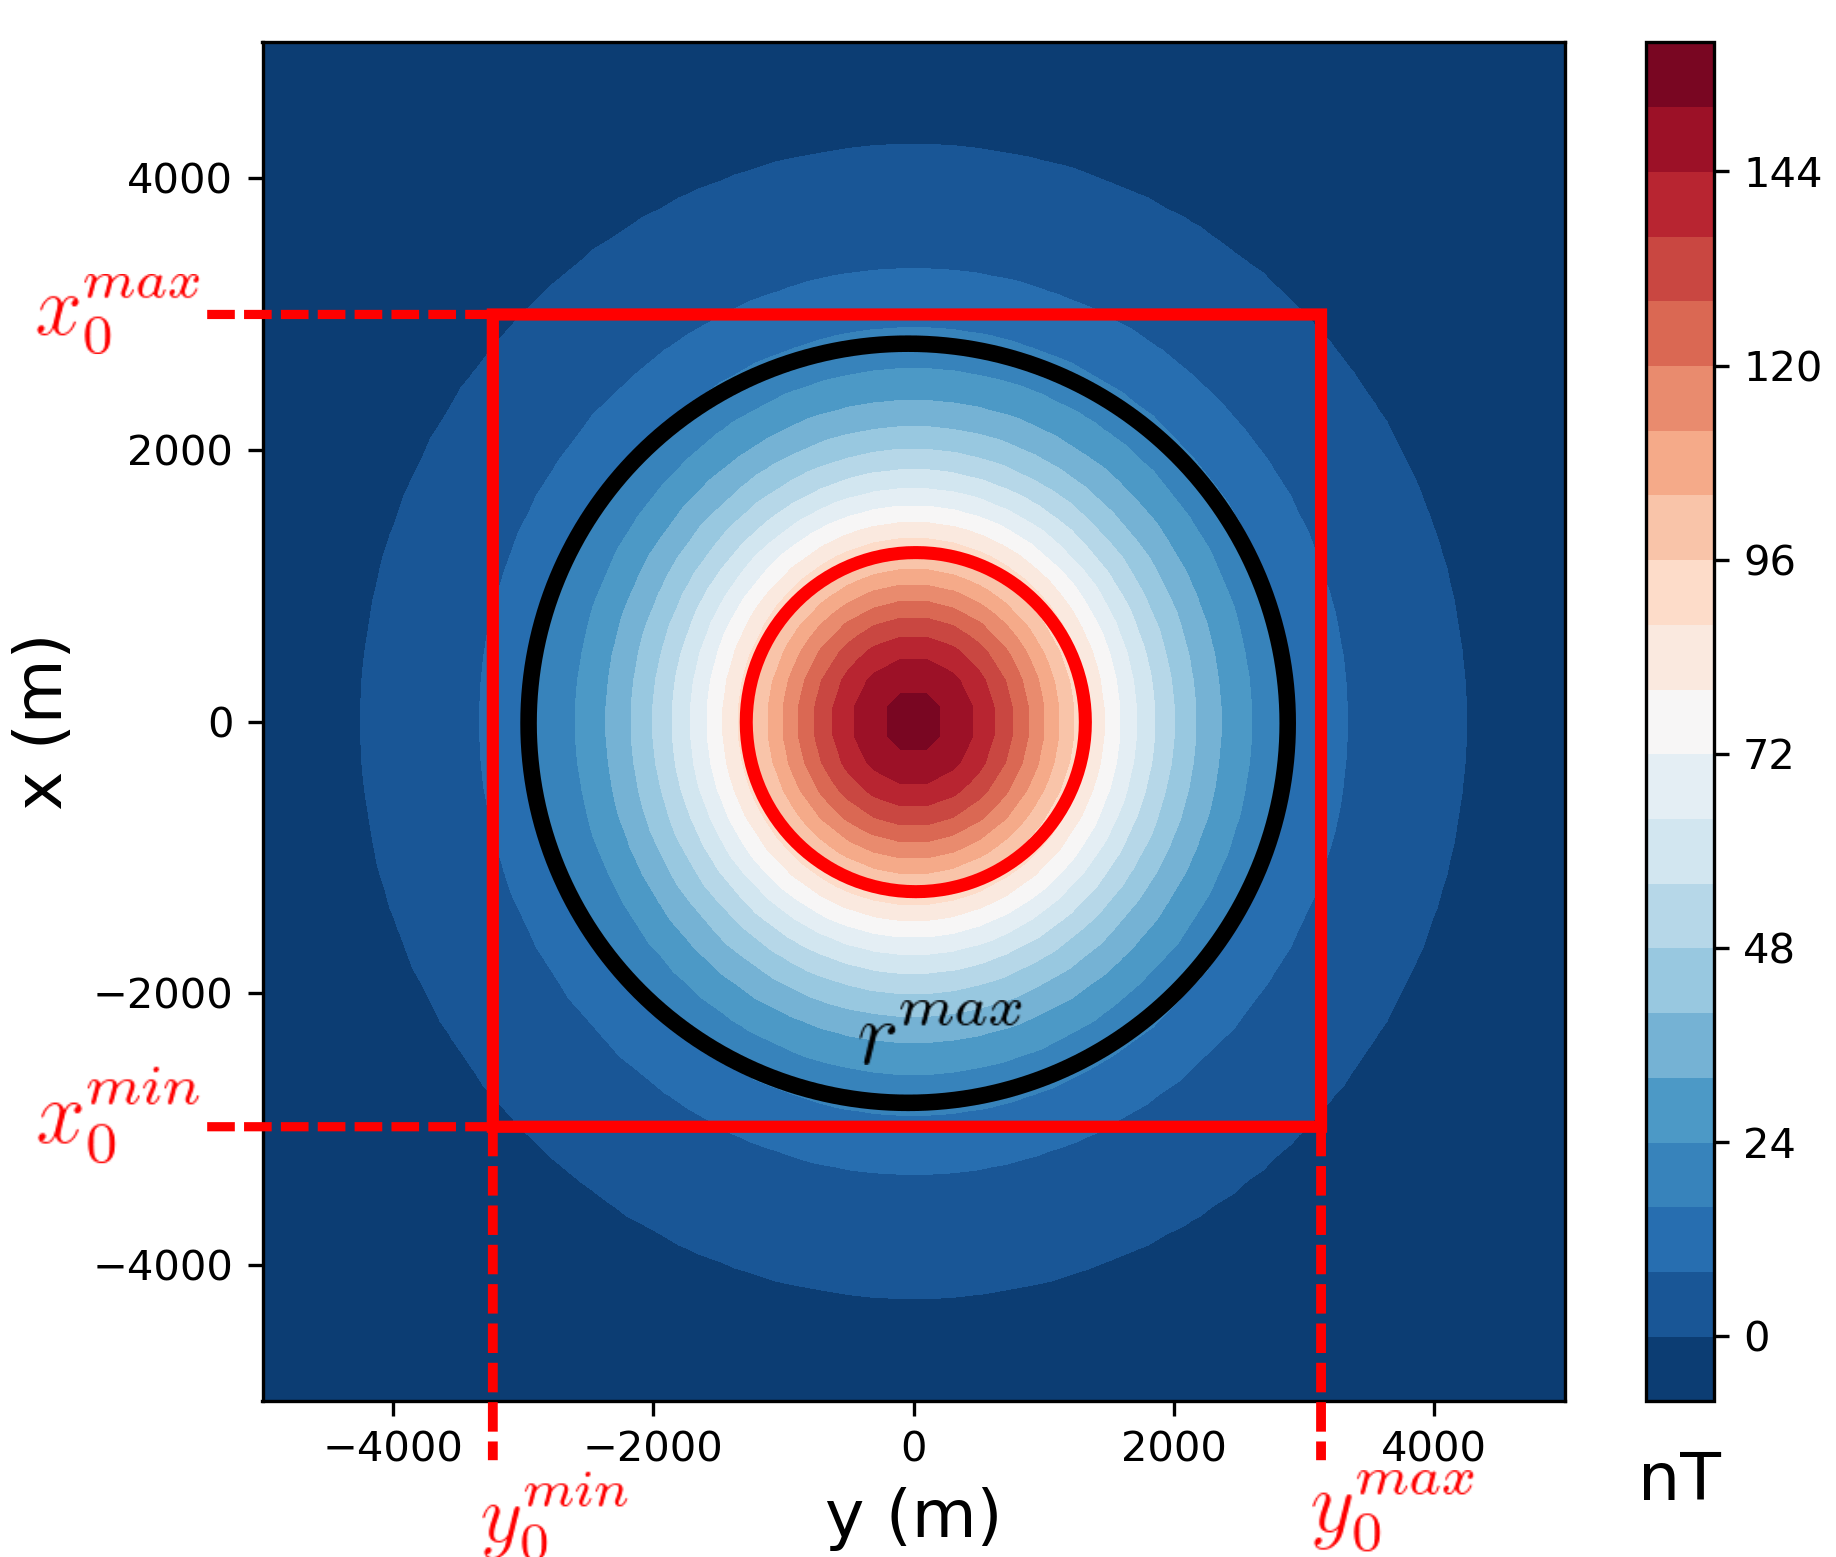
\includegraphics[scale=0.6]{rtp-example.png}
	\caption{Exemplo ilustrativo de anomalia de campo total reduzida ao polo para a definição dos limites do vínculo de desigualdades e aproximação inicial. O círculo preto representa o valor máximo $ r^{max} $ para os raios $r_j^k$, $j=1,\dots ,V$, $k=1,\dots ,L$. O retângulo vermelho representa a área composta pelos valores mínimos ($ x_0^{min} $ e $ y_0^{min} $) e máximos ($ x_0^{max} $ e $ y_0^{max} $) das coordenadas Cartesianas horizontais $ x_0^k $ e $ y_0^k $ da origem $ O^k $. Já o círculo vermelho representa o raio $r_j^k$ da aproximação inicial cilíndrica $ \hat{\mathbf{p}}_0 $.}
	\label{fig:rtp}
\end{figure}

Para definir o raio e as coordenadas horizontais do centro da aproximação inicial cilíndrica $ \hat{\mathbf{p}}_0 $, é escolhida a área circular que compreende a região onde a anomalia RTP é positiva e possui seu máximo.
O ideal aqui é que o raio da aproximação inicial $ \hat{\mathbf{p}}_0 $ coincida com a região de máximo gradiente da anomalia RTP, ou seja, onde se encontra a variação máxima desse dado, que pode indicar os limites laterais da fonte alvo \citep{baranov1957}.
Essa definição não exige um rigor matemático muito acurado.
Depois de definir o raio e as coordenadas Cartesianas horizontais do centro da aproximação cilíndrica inicial $ \hat{\mathbf{p}}_0 $, devem ser escolhidos sua espessura de modo que a aproximação inicial seja mais profunda que a extensão vertical esperada fonte alvo.
A próxima etapa consiste em um modelagem direta da anomalia de campo total (Eq. \ref{eq:predicted-data-i}) com o intuito de ajustar o volume e definir os intervalos para a sua intensidade de magnetização total $m_{0}$ e a profundidade do topo $z_{0}$, as quais ajustam preliminarmente o dado observado $ \mathbf{d}^o $.
A Figura \ref{fig:prefit} exemplifica esse ajuste preliminar dos dados observados.
Note que essa modelagem direta é realizada antes de iniciar o processo de inversão e 
que o corpo cilíndrico resultante pode produzir um ajuste impreciso dos dados.

%FIGURA
\begin{figure}[!htb]
	\centering
	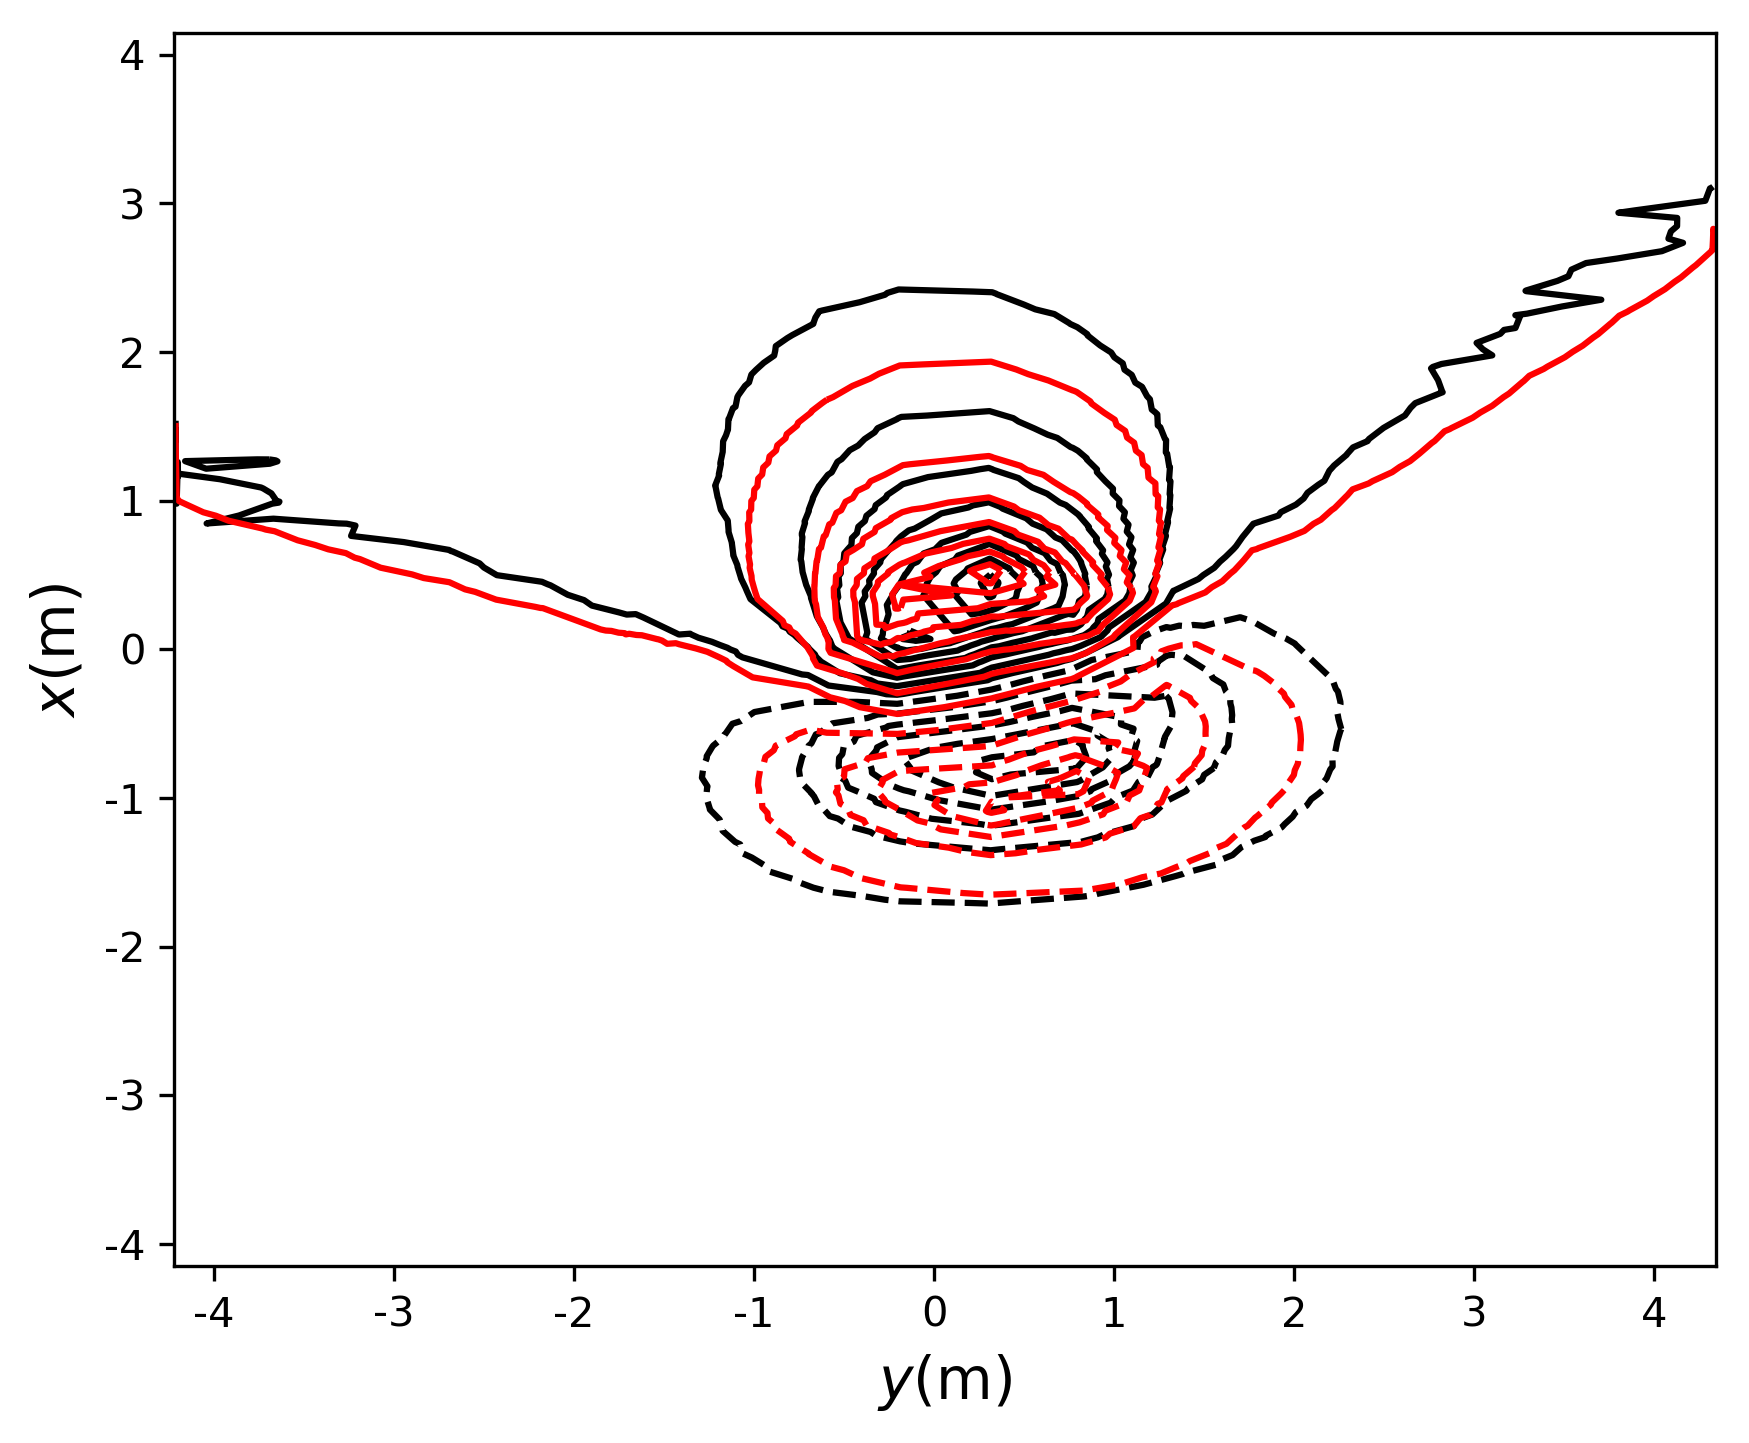
\includegraphics[scale=0.7]{prefitting.png}
	\caption{Exemplo ilustrativo de um ajuste preliminar entre anomalia de campo total observada (linhas pretas) e os dados produzidos pela da aproximação inicial $ \hat{\mathbf{p}}_0 $ (linhas vermelhas). Linhas contínuas representam dados positivos e linhas tracejadas representam dados negativos.}
	\label{fig:prefit}
\end{figure}

\section{Escolha dos pesos $\alpha_{1}-\alpha_{5}$}

Atribuir valores aos pesos $ \alpha_{\ell} $ (Eq. \ref{eq:gamma}) é uma etapa muito importante deste método.
Entretanto, não existe uma regra analítica para definí-los e seus valores podem ser muito dependentes das características particulares da área onde o método está sendo aplicado \cite[]{silva-2001,bastos-2020}.

Neste ponto, vale ressaltar que os pesos $ \alpha_{\ell}$ (eq. \ref{eq:gamma}) são quantidades com dimensão.
Note que as unidades da função data-misfit para a norma-2 e norma-1 dos resíduos (Eqs. \ref{eq:L2_misfit} e \ref{eq:L1_misfit}) são nT$^2$ e nT, respectivamente.
E as funções dos vínculos (Eqs. \ref{eq:phi1}, \ref{eq:phi2}, \ref{eq:phi3}, \ref{eq:phi4} e \ref{eq:phi5}) possuem unidade de m$^2$.
Por essa razão, a unidade dos pesos $ \alpha_{\ell} $ (Eq. \ref{eq:gamma}) é nT$^{2}/$m$^{2}$ para quando a função data-misfit é a norma-2 dos resíduos (Eq. \ref{eq:L2_misfit}) e nT$/$m$^{2}$ para o caso da utilização da norma-1 dos resíduos (Eq. \ref{eq:L1_misfit}).

A dimensão física dos pesos $ \alpha_{\ell}$ torna a definição de seus valores muito depende da escala da área de estudo,
das dimensões da fonte alvo e da configuração dos dados observados.
Com o íntúito de remover ou amenizar esta dependência, realiza-se a seguinte normalização sobre $ \alpha_{\ell} $:
\begin{equation}\label{eq:alphas}
\alpha_{\ell} = \tilde{\alpha}_\ell \frac{E_\phi}{E_\ell}, \quad \ell = 1,\dots, 5,
\end{equation}
em que $\tilde{\alpha}_\ell$ é um escalar positivo e $ E_\phi/E_\ell $ é um fator de normalização que permite que os $\tilde{\alpha}_\ell$ sejam independentes de unidades físicas utilizadas.
Nesta equação, $ E_\ell $ representa o traço da matriz Hessiana $\mathbf{H}_{\ell}$ (eqs \ref{eq:phi1_gh}, \ref{eq:phi2_gh}, \ref{eq:phi3_gh}, \ref{eq:phi4_gh} e \ref{eq:phi5_gh}) da $ \ell $-ésima função de vínculo $\varphi_{\ell}(\mathbf{p})$ (eqs \ref{eq:phi1}, \ref{eq:phi2}, \ref{eq:phi3}, 
\ref{eq:phi4} e \ref{eq:phi5}).
A constante $E_\phi$ é o traço da matriz Hessiana $\mathbf{H}_{\phi}(\hat{\mathbf{p}}_{(0)})$ da função data-misfit $\phi(\mathbf{p})$ (Eqs. \ref{eq:L2_misfit} e \ref{eq:L1_misfit}) computada com a aproximação inicial $\hat{\mathbf{p}}_{(0)}$ para o vetor de parâmetros $ \mathbf{p} $ (Eq. \ref{eq:p-vector}) no início do algoritmo de inversão.
Note que o traço da matriz Hessiana $\mathbf{H}_{\ell}$ é adimensional e o traço da matriz Hessiana $\mathbf{H}_{\phi}(\hat{\mathbf{p}}_{(0)})$ tem unidade de nT$^{2}/$m$^{2}$ para a norma-2 e nT$ / $m$ ^2 $ para a norma-1.
Logo, os escalares positivos $\tilde{\alpha}_\ell$ na Equação \ref{eq:alphas} são quantidades adimensionais.

De acordo com essa estratégia empírica, os pesos $ \alpha_{\ell} $ 
(Eq. \ref{eq:gamma}) são redefinidos usando os escalares positivos $\tilde{\alpha}_\ell$ (eq. \ref{eq:alphas}), os quais são independentes de unidades físicas e menos dependentes de fatores como a escala da área de estudo, dimensões da fonte alvo e configuração dos dados observados.

\section{Considerações práticas}

Os valores atribuídos ao pesos adimensionais $\tilde{\alpha}_{1} - \tilde{\alpha}_{5}$ (eq. \ref{eq:alphas}) impactam significativamente os modelos estimados e não podem ser automaticamente escolhidos sem o julgamento do intérprete.
Baseado em \cite{bastos-2020}, este trabalho sugere alguns procedimentos para a escolha desses parâmetros.

Os parâmetros $\tilde{\alpha}_1$ e $\tilde{\alpha}_2$ impõem informação a priori na forma da seção horizontal dos prismas.
O primeiro força todos os prismas a terem uma seção horizontal circular, enquanto o segundo força todos os prismas a terem uma seção horizontal parecida.
Geralmente, seus valores variam de $10^{-5}$ a $10^{-3}$ e diferem entre si de uma ordem de grandeza, no máximo.
O parâmetro $\tilde{\alpha}_3$ também varia de $10^{-5}$ a $10^{-3}$ e controla a posição relativa dos prismas adjacentes que formam o modelo interpretativo.
Um valore alto privilegia um corpo estimado vertical, enquanto um valor pequeno tende a gerar um corpo estimado inclinado.

O parâmetro $\tilde{\alpha}_4$ possui um significado puramente matemático e é usado somente para estabilizar as soluções do problema inverso.
Seu valor é escolhido como o menor possível.
O parâmetro $\tilde{\alpha}_7$ controla a extensão vertical total do corpo estimado.
Quanto maior é o seu valor, mais rasa é a profundidade da base estimada e vice versa.
Uma regra geral é começar com os valores iniciais $\tilde{\alpha}_1 = 10^{-4}$, $\tilde{\alpha}_2 = 10^{-4}$, $\tilde{\alpha}_3 = 10^{-4}$, $\tilde{\alpha}_4 = 10^{-7}$ e $\tilde{\alpha}_5 = 10^{-5}$, e mudá-los para refinar os resultados.
Finalmente, é importante enfatizar que  $\tilde{\alpha}_1 - \tilde{\alpha}_5$ (Eq. \ref{eq:alphas}) não são alterados ao longo das iterações do algortimo de inversão.

\section{Critério para escolha da melhor solução}
\label{sec:criterio}

A escolha da melhor entre as soluções L2 e L1 é feita comparando-se os valores das funções dos vínculos $ \varphi_\ell $ (Equações \ref{eq:phi1}, \ref{eq:phi2}, \ref{eq:phi3}, \ref{eq:phi4} e \ref{eq:phi5}) multiplicados pelos pesos normalizados $ \alpha_\ell $, $ \ell=1,\dots,5 $ (Equação \ref{eq:alphas}) para cada solução.
A melhor solução é definida como aquela que possui os menores valores dos produtos $ \alpha_\ell \varphi_\ell  $, $ \ell=1,\dots,5 $.
Note que, quando este produto assume um valor pequeno, isso significa que a informação a priori imposta pelo $ \ell $-ésimo vínculo foi bem incorporada à solução final.
Por exemplo, uma solução cilíndrica vai apresentar valores de $ \varphi_1 $, $ \varphi_2 $ e $ \varphi_3 $ iguais a zero independentemente do valor de seus respectivos pesos normalizados $ \alpha_1 $, $ \alpha_2 $ e $ \alpha_3 $, uma vez que todos os raios $ r^k_j $, $ j=1, \dots, V $, $ k=1,\dots,L $, e todas as coordenadas Cartesianas horizontais $ (x^k_0, y^k_0) $ das origens $ O^k $ de todos os $ L $ prismas que compõem o modelo interpretativo serão iguais (Eqs. \ref{eq:phi1}, \ref{eq:phi2} e \ref{eq:phi3}).
Portanto, neste trabalho, a melhor solução é definida como aquela que melhor incorpora as informações a priori em comparação à outra.